\documentclass[a4paper,12pt,svgnames]{report}
\usepackage[utf8]{inputenc}
\usepackage[width=17cm,height=27cm,includeheadfoot]{geometry}
\usepackage[pdftex,colorlinks=true]{hyperref}
\usepackage{fancyhdr,lastpage}
\usepackage{tabularx}
\usepackage[table]{xcolor}
\usepackage{titlesec, blindtext, color}
\usepackage{wrapfig, graphicx}

%opening
\title{SocInfo2012}
\author{$\;$}

\titleformat{\chapter}[hang]{\Huge\bfseries}{$\;$}{0pt}{}{}
\titleformat{\section}[display]{\Large\bfseries}{$\;$}{0pt}{}{}

\newcounter{sectocnonumdepth}
\setcounter{sectocnonumdepth}{1}

% Trick to format tables
\newcommand{\ncell}[2][X]{%
\begin{tabularx}{0.69\linewidth}[#1]{@{}X@{}}#2\end{tabularx}%
}
  

  
\begin{document}
\pagestyle{fancy}
\renewcommand{\headrulewidth}{1pt}
\renewcommand{\footrulewidth}{1pt}
\renewcommand{\headheight}{15pt}
\fancyhead[L]{SocInfo2012}
\fancyhead[R]{The 4th International Conference on Social Informatics}
\fancypagestyle{plain}{
	\renewcommand{\headrulewidth}{1pt}
	\renewcommand{\footrulewidth}{1pt}
}

\maketitle

\tableofcontents

\chapter{Preface}

\chapter{Committees}

\chapter{Sponsors}

\chapter{Practical details}
\section{Wi-Fi access}
\section{Maps}

\chapter{Programme Overview}

NOTE: We should indicate the rooms in the tables
\begin{center}
\bgroup
\def\arraystretch{1.5}
\begin{tabularx}{.9\linewidth}{|c|X|X|}
\hline
\multicolumn{3}{|c|}{\textbf{Wednesday, December 5}}\\
\hline
08:00 $\rightarrow$ 18:00 & \multicolumn{2}{c|}{Registration}\\
\hline
08:45 $\rightarrow$ 09:00 & \multicolumn{2}{c|}{Conference opening}\\
\hline
09:00 $\rightarrow$ 10:00 & \multicolumn{2}{c|}{\cellcolor{green!20}
\ncell{Keynote by Andreas Ernst:\\About the Why? and the How? of psychologically
plausible agents}}\\
\hline
10:00 $\rightarrow$ 10:30 & \multicolumn{2}{c|}{Break}\\
\hline
10:30 $\rightarrow$ 12:30 & \multicolumn{2}{c|}{\cellcolor{blue!20}Session
1: Social Graph, Social Influence and Viral Marketing}\\
\hline
12:30 $\rightarrow$ 14:00 & \multicolumn{2}{c|}{Lunch break}\\
\hline
14:00 $\rightarrow$ 16:00 & \multicolumn{2}{c|}{\cellcolor{blue!20}Session 2:
Recommendation and Crowd Computing }\\
\hline
16:00 $\rightarrow$ 16:30 & \multicolumn{2}{c|}{Break}\\
\hline
16:30 $\rightarrow$ 18:00 & \cellcolor{red!20} Tutorial 1: Supporting
sociological theories with social media data mining  &
\cellcolor{red!20} Tutorial 2: Online Social Experiments with nodeGame \\
\hline
\end{tabularx}
\egroup
\end{center}

\begin{center}
\bgroup
\def\arraystretch{1.5}
\begin{tabularx}{.9\linewidth}{|c|X|}
\hline
\multicolumn{2}{|c|}{\textbf{Thursday, December 6}}\\
\hline
09:00 $\rightarrow$ 10:00 & \multicolumn{1}{c|}{\cellcolor{green!20}
\ncell{Keynote by Bernardo Huberman:\\Big Data and the Attention Economy}}\\
\hline
10:00 $\rightarrow$ 10:30 & \multicolumn{1}{c|}{Break}\\
\hline
10:30 $\rightarrow$ 12:30 & \multicolumn{1}{c|}{\cellcolor{blue!20}Session
3: Sentiment Analysis and Trust}\\
\hline
12:30 $\rightarrow$ 14:00 & \multicolumn{1}{c|}{\cellcolor{red!20}Buffer lunch
with poster/demo session}\\
\hline
14:00 $\rightarrow$ 16:00 & \multicolumn{1}{c|}{\cellcolor{blue!20}Session 4:
Social Tagging and Discovery}\\
\hline
16:00 $\rightarrow$ 16:30 & \multicolumn{1}{c|}{Break}\\
\hline
16:30 $\rightarrow$ 18:00 & \multicolumn{1}{c|}{\cellcolor{red!20}
\ncell{Tutorial 3: Human activity and
mobility patterns: measurements, models,\\ and implications }} \\
\hline
\end{tabularx}
\egroup
\end{center}

\begin{center}
\bgroup
\def\arraystretch{1.5}
\begin{tabularx}{.9\linewidth}{|c|X|}
\hline
\multicolumn{2}{|c|}{\textbf{Friday, December 7}}\\
\hline
09:00 $\rightarrow$ 10:00 & \multicolumn{1}{c|}{\cellcolor{green!20}
\ncell{Keynote by Dirk Helbing:\\ From Computational Social Science to
Socio-Inspired Technology to Artificial Societies}}\\
\hline
10:00 $\rightarrow$ 10:30 & \multicolumn{1}{c|}{Break}\\
\hline
10:30 $\rightarrow$ 12:30 & \multicolumn{1}{c|}{\cellcolor{blue!20}Session 5:
Community Detection and Evolution}\\
\hline
12:30 $\rightarrow$ 14:00 & \multicolumn{1}{c|}{Lunch break}\\
\hline
14:00 $\rightarrow$ 16:00 & \multicolumn{1}{c|}{\cellcolor{blue!20}Session 6:
Social Informatics and Applications }\\
\hline
16:00 $\rightarrow$ 16:30 & \multicolumn{1}{c|}{Break}\\
\hline
16:30 $\rightarrow$ 18:00 & \multicolumn{1}{c|}{\cellcolor{red!20}
Plenary Panel} \\
\hline
\end{tabularx}
\egroup
\end{center}

\chapter{Keynote speakers}
\section{About the Why? and the How? of psychologically plausible agents}

\noindent \textit{Prof. Dr. Andreas Ernst}

\noindent December 5, 09:00-10:00
\\

\noindent To deepen the analysis and understanding of human behaviour by
using artificial societies, a credible modelling of agents and their decision
processes is needed. Such a deep analysis can be informed by the psychological
knowledge about processes and triggers of specific behaviours, given the
interaction between an agent’s environment and some individual preference set.
This requires a framework capable of handling a high number of deep,
heterogeneous agents, together with their individual networks.

In this presentation, a software framework is presented that aims at providing
psychological plausibility to the modelling of so-called citizen agents. It
fills the gap between (flat) agent frameworks without any built-in psychological
foundations on the one hand and full-fledged (deep) cognitive architectures on
the other hand, the latter being computationally too intensive to be of any use
in larger scale problems. The framework provides prefabricated components of an
agent’s decision process like perception, memory, different modes of decision
making, basic learning algorithms, or social influence. Each of these components
is based on appropriate psychological empirical results or theories.

Using this framework, together with specifically gathered data, an agent’s
interaction with other agents, technology, or the natural environment can be
investigated. Examples include energy use, innovation adoption, or helper
networks. Besides the emerging macro phenomena, their micro foundation lying in
the individual preferences and processes are important data produced by the
framework. Individual, local perception of the technical or physical environment
and the information of the individual social network are crucial in determining
an agent’s behaviour.

To model larger amounts of social data, with a higher number of agents together
with their networks, the sociological concept of lifestyles can be used as a
classifying element, and as a bridge to upscale the individual data to the agent
set.\\

\begin{wrapfigure}[13]{l}{11em}
  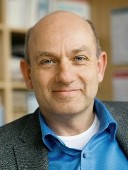
\includegraphics{andreas_ernst}
\end{wrapfigure}
\noindent\textbf{Andreas Ernst} achieved his psychology Diplom
degree with a focus on psychology of knowledge/cognitive science in 1988. He
finished his PhD—entitled "Social knowledge as basis of decisions in conflict
situations"—in 1993. Until 1999 he was assistant professor at the Institute of
Psychology, University of Freiburg i. Br. and in the same year he finished his
postdoctoral lecture qualification under the title: "Information dilemmas and
the use of natural resources". After another three years at the Institute of
Psychology, University of Freiburg i.Br. he became full professor for
Environmental Systems Analysis at the Center for Environmental Systems Research
of the University of Kassel. He also heads the Graduate Program
"Man-Environment-Systems" (ProMUS) and is the current president of the European
Social Simulation Association (ESSA). Prof. Dr. Andreas Ernst is co-editor of
the book series "Social Science Simulations" of the Metropolis-Verlag.


\section{Big Data and the Attention Economy}

\noindent \textit{Bernardo A. Huberman}

\noindent December 6, 09:00-10:00
\\

\noindent The advent of the web has led to an ever expanding ocean of data whose
outlines are hard to discern but its effects are easy to feel. It reflects a
societal change that is both global and daunting at the same time. Global
because it encompasses content created by people seeking attention and
information from all over the world without much awareness of privacy issues.
And daunting since it is hard to discern what to pay attention to when
confronted with such flood of content.

This talk will describe the effects that the attention economy has on the
production and consumption of big data and the opportunities that big data
offers about learning the behavior of large groups of people and the design of
novel socially attentive systems. It will also address the questions that big
data poses about privacy and how markets for private data can restore a sense of
control to most users of the web.\\

\begin{wrapfigure}[13]{l}{11em}
  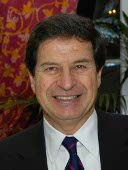
\includegraphics{bernardo_huberman}
\end{wrapfigure}

\noindent\textbf{Bernardo A. Huberman} is a Senior HP Fellow and director of
the Social Computing Research Group at HP Labs, which focuses on methods for
harvesting the collective intelligence of groups of people in order to realize
greater value from the interaction between users and information. Huberman’s
main research focus is on the relationship between local actions and the global
behavior of large, distributed systems. Areas of exploration include distributed
knowledge, social organizations and the economics of attention. Much of
Huberman's research has concentrated on the World Wide Web, with an emphasis on
the dynamics of its growth and use. This work helped uncover the nature of
electronic markets, the detailed structure of the web and the laws governing the
way people surf for information. One of the originators of the field of ecology
of computation, Huberman recently published the book, "The Laws of the Web:
Patterns in the Ecology of Information," with MIT Press.

\section{From Computational Social Science to Socio-Inspired Technology to
Artificial Societies}

\noindent \textit{Dirk Helbing}

\noindent December 7, 09:00-10:00
\\

\noindent  What can we learn from the way society is organized? What are the
underlying principles? How can we use them to design new technological systems?

Along the lines of these guiding questions, I will start with models of
pedestrians and crowds, and the applications in logistics and traffic light
control they have inspired.

It will be shown that self-organization is a wide-spread principle underlying
the emergence of social coordination, cooperation, and social norms. These
phenomena can now be dynamically modeled based on evolutionary principles, which
are transferable to ICT systems as well. I will also discuss, how and why the
wrong kinds of system designs can lead to breakdowns of traffic flows,
cooperation, or financial markets. It will be argued that the theory of complex
systems can help to provide an explanatory understanding of desirable and
undesirable cascading effects and guidelines for the design of socially
interactive systems (such as the 'ecosystem' of financial trading algorithms).
\\

\begin{wrapfigure}[13]{l}{11em}
  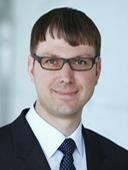
\includegraphics{dirk_helbing}
\end{wrapfigure}

\noindent\textbf{Dirk Helbing} has worked as Managing Director of the Institute
for Transport \& Economics at TU Dresden and is now Professor of Sociology, in
particular of Modeling and Simulation at ETH Zurich. Having studied physics and
mathematics, he investigates complex social, economic, and transport systems
with methods from statistical physics, individual-based models, and behavioral
experiments. Helbing is well-known for the social force model, in particular its
application to self-organization phenomena in pedestrian crowds. Besides the
slower-is-faster effect, he introduced the freezing-by-heating effect and the
phase diagram of congested traffic states. Recent work applies principles of
collective intelligence and dynamics to the optimization of freeway and urban
traffic flows. In game theory, Helbing proposed a microscopic foundation of
evolutionary game theory and studied self-organized behavioral conventions early
on. His current work develops socio-inspired technologies and investigates the
role of success-driven motion for the establishment of cooperation among selfish
individuals.

\chapter{Abstracts per session}

\section{Session 1: Social Graph, Social Influence and Viral Marketing}

\begin{itemize}
\item \textbf{Connecting with Active People Matters: The Influence of an Online
Community on Physical Activity Behavior}

\textit{Maartje Groenewegen, Dimo Stoyanov, Dirk Deichmann and Aart van
Halteren}

This paper discusses the impact of online social networks as means to motivate
people to become more physically active. Based on a data set from 4333
participants we show that the activity level of people that participated in the
online community (for 14 weeks) is significantly higher compared to people that
choose not to become a member of that community. Detailed analyses show that the
number of contacts in the online community does not have a significant effect on
the physical activity level while network density even has a significant,
negative effect. On the other hand, the activity level of a participant is
higher when his or her friends also have a high average activity level. This
effect is even higher when a participant's amount of friends
increases.Theoretical and managerial implications concerning the impact of
online social networks on offline behavior are discussed. 

\item \textbf{The Multidimensional Study of Viral Campaigns as Branching
Processes}

\textit{Jaroslaw Jankowski, Radoslaw Michalski and Przemyslaw Kazienko}

Viral campaigns on the Internet may follow variety of models, depending on the
content, incentives, personal attitudes of sender and recipient to the content
and variety of other factors. Due to the fact that the knowledge of the campaign
specifics is essential for the campaign managers, researchers are constantly
evaluating models and real-world data. The goal of this article is to present
the new knowledge obtained from studying two viral campaigns that took place in
a virtual world which followed the branching process. The results show that it
is possible to reduce the time needed to estimate the model parameters of the
campaign and, moreover, some important aspects of time-generations relationship
are presented.

\item \textbf{A Model to Represent Human Social Relationships in Social Network
Graphs}

\textit{Marco Conti, Andrea Passarella and Fabio Pezzoni}

Human social relationships are a key component of emerging complex techno-social
systems such as socially-centric platforms based on the interactions between
humans and ICT technologies. Therefore, the models of human social relationships
are fundamental to characterise these systems and study the performance of
socially-centric platforms depending on the social context where they operate.
The goal of this paper is presenting a generative model for building synthetic
human social network graphs where the properties of social relationships are
accurately reproduced. The model goes well beyond a binary approach, whereby
edges between nodes, if existing, are all of the same type. It sets the
properties of each social link, by incorporating fundamental results from the
anthropology literature. The synthetic networks it generates accurately
reproduce both the macroscopic structure (e.g., its diameter and clustering
coefficient), and the microscopic structure (e.g., the properties of the tie
strength of individual social links) of human social networks. We compare
generated networks with a large-scale social network data set, validating that
the model is able to produce graphs with the same structural properties of
human-social-network graphs. Moreover, we characterise the impact of the model
parameters on the synthetic graph properties.


\item \textbf{Interpolating between Random Walks and Shortest Paths: a Path
Functional Approach}

\textit{Francois Bavaud and Guillaume Guex}

General models of network navigation must contain a deterministic or drift
component, encouraging the agent to follow routes of least cost, as well as a
random of diffusive component, enabling free wandering. This paper proposes a
thermodynamic formalism involving two path functionals, namely an energy
functional governing the drift and an entropy functional governing the
diffusion.\\
A freely adjustable parameter, the temperature, arbitrates between the
conflicting objectives of minimising travel costs and maximising spatial
exploration. The theory is illustrated on various graphs and various
temperatures. The resulting optimal paths, together with presumably new
associated edges and nodes centrality indices, are analytically and numerically
investigated. 

\item \textbf{Studying Paths of Participation in Viral Diffusion Process within
Virtual Chat Environment}

\textit{Jaroslaw Jankowski, Sylwia Ciuberek, Anita Zbieg and Radoslaw Michalski}

Authors propose a conceptual model of participation in viral diffusion process
composed of four stages: awareness, infection, engagement and action. To verify
the model it has been applied and studied in the virtual social chat environment
settings. The study investigates the behavioural paths of actions that reflect
the stages of participation in the diffusion and presents shortcuts, that lead
to the final action – the attendance in a virtual event. The results show that
the participation in each stage of the process increases the probability of
reaching the final action. Nevertheless, the majority of users involved in the
virtual event did not go through each stage of the process but followed the
shortcuts. That suggests that the viral diffusion process is not necessarily a
linear sequence of human actions but rather a dynamic system.


\item \textbf{How Influential are You: Detecting Influential Bloggers in a
Blogging Community}

\textit{Imrul Kayes}

The emergence of advanced web 2.0 technologies has created a new horizon for
previously known information consumer, enabled them to produce information on
the web through novel and innovative inter- active applications such as blogs. A
Blog is a virtual media on the web where users commonly referred as bloggers
publish their context aware information. Bloggers write blog posts, express a
preference through likes and dislikes, voice their opinions, participate debate,
report news, and form virtual communities of similar interest groups on the
Blogosphere. Bloggers interactions on blogosphere mimic, to some extent, real
world interaction. Inspired by the high impact of the influential individuals in
a real world community, we study a contemporary problem of identifying
influential bloggers at a blogging platform. We model bloggers influence based
upon a wide range of centrality measurements and quantify influence strength. We
conduct experiments with data from a real world blogging platform, discover
multi-facets of the problem of identifying influential bloggers, and discuss
plausible methods. Our study reveals that some bloggers span MEGA influence on
fellow bloggers and there is some degree of correlation between the methods that
are used along the uncovering process.


\item \textbf{Dark Retweets: Investigating Non-Conventional Retweeting Patterns}

\textit{Norhidayah Azman, David Millard and Mark Weal}

Retweets are an important mechanism for recognising propagation of information
on the Twitter social media platform. However, many retweets do not use the
official retweet mechanism, or even community established conventions, and these
"dark retweets" are not accounted for in many existing analysis. In this paper,
a comprehensive matrix of tweet propagation is presented to show the different
nuances of retweeting, based on seven characteristics: whether it is
proprietary, the mechanism used, whether it is directed to followers or
non-followers, whether it mentions other users, if it is explicitly propagating
another tweet, if it links to an original tweet, and what is the audience it is
pushed to. Based on this matrix and two assumptions of retweetability, the
degrees of a retweet's "darkness" can be determined. This matrix was evaluated
over 2.3 million tweets and it was found that dark retweets amounted to 12.86\%
(for search results less than 1500 tweets per URL) and 24.7\% (for search
results including more than 1500 tweets per URL) respectively. By extrapolating
these results with those found in existing studies, potentially thousands of
retweets may be hidden from existing studies on retweets.

\end{itemize}

\section{Session 2: Recommendation and Crowd Computing}
\begin{itemize}
\item \textbf{A Framework for the Design and Synthesis of Coordinated Social
Systems}

\textit{Wynn Sterling, Christophe Giraud-Carrier and Teppo Felin}

This paper describes how a nascent collective of individuals can coalesce into a
complex social system. The systematic study of such scenarios requires a
mathematical framework within which to model the behavior of the individual
members of the collective. As individuals interact, they develop social
relationships and exchange resources -- that is, they develop social capital
that quantifies the value of social influence that individuals exert on each
other. Social capital can be expressed via conditional preference orderings for
each individual. Conditional preferences reflect the influence relationships of
an interacting social collective. Conditional preference orderings can then be
aggregated via conditional game theory to form a concordant utility that
provides an emergent group-level ordering of the harmony of interests of the
members of the collective. We can thus develop a complete social model that
takes into consideration all social relationships as they propagate through the
system. Solution concepts can then be defined that simultaneously account for
both group-level and individual-level interests.

\item \textbf{CrowdLang: A Programming Language for the Systematic Exploration
of Human Computation Systems}

\textit{Patrick Minder and Abraham Bernstein}

Human computation systems are often the result of extensive lengthy
trial-and-error refinements. What we lack is an approach to systematically
engineer solutions based on past successful patterns.\\
In this paper we present the CrowdLang programming framework for engineering
complex computation systems incorporating large crowds of networked humans and
machines incorporating a library of known interaction patterns. We evaluate
CrowdLang by programming a German- to-English translation program incorporating
machine translation and a monolingual crowd.\\
The evaluation shows that CrowdLang is able to simply explore a large design
space of possible problem solving programs with the simple variation of the used
abstractions. In an experiment involving 1918 different human actors, we show
that the resulting translation program significantly outperforms a pure machine
translation in terms of adequacy and fluency whilst translating more than 30
pages per hour and approximates the human-translated gold-standard to 75\%.


\item \textbf{A multi-view content-based user recommendation scheme for
following users in Twitter}

\textit{Milen Chechev and Petko Georgiev}

This paper describes recommendation techniques that help users to find
potentially interesting people to follow at Twitter. The explored techniques are
based on a confirmed assumption that the recent activity of users is indicative
of their latest friend preferences. Several content-based recommendation
strategies are explored, compared and tested. Among them the foundations for a
novel hybridization framework are provided and a multi-view approach towards
modeling user profiles is considered. The training and test database is crawled
with real users and tweets from the Twitter network. A non-standard evaluation
scheme is applied in an offline testing context for the various algorithms.
Con-clusions are drawn as to the viability, relative predictive power and
accuracy of the recommendation approaches. 

\item \textbf{A Survey of Recommender Systems in Twitter}

\textit{Su Mon Kywe, Ee-Peng Lim and Feida Zhu}

Twitter is a social information network where short messages or tweets are
shared among a large number of users through a very simple messaging mechanism.
With a population of more than 100M users generating more than 300M tweets each
day, Twitter users can be easily overwhelmed by the massive amount of
information available and the huge number of people they can interact with. To
overcome the above information overload problem, recommender systems can be
introduced to help users make the appropriate selection. So far, researchers
have began to study recommendation problems in Twitter but their works usually
address individual recommendation tasks. There is so far no comprehensive survey
for the realm of recommendation in Twitter to categorize the existing works as
well as to identify areas that need to be further studied. The paper therefore
aims to fill this gap by introducing a taxonomy of recommendation tasks in
Twitter, and to use the taxonomy to describe the relevant works in recent years.
The paper further presents the datasets and techniques used in these works.
Finally, it proposes a few research directions for recommendation tasks in
Twitter.

\item \textbf{Swayed by Friends or by the Crowd?}

\textit{Zeinab Abbassi, Christina Aperjis and Bernardo Huberman}

We have conducted three empirical studies of the effects of friend
recommendations and general ratings on how online users make choices.
We model and quantify how a user deciding between two choices trades off an
additional rating star with an additional friend's recommendation when selecting
an item.\\
We find that negative opinions from friends are more influential than positive
opinions, and people exhibit ``more random'' behavior in their choices when the
decision involves less cost and risk. Our results are quite general in the sense
that people across different demographics trade off recommendations from friends
and ratings from the general public in a similar fashion. 

\item \textbf{Quality assessment of user comments on mobile platforms
considering channel of activation and platform design}

\textit{Christopher Fröch and Martin Schumann}

In this paper we present the results of an experimental three-steps-study
concerning quality assessment of product reviews. As reviews and comments on
products and services are gaining importance in the context of purchasing
decisions providers of review platforms are seeking for ways to improve the
quality of their platforms. In the presented study user expectations regarding
quality of comments were collected as well as reader perceptions of quality.
Additionally a thorough text analysis of experimentally obtained product reviews
was conducted. The main results of this research were that quality expectations
do not necessarily lead towards good quality comments provided by the same
person. Moreover it could be observed that the combination of text and star
rating is preferred by people and also will lead to better understandability of
resulting comments. The channel of activation, NFC or QR codes did not cause any
significant difference considering comment quality or appropriate platform.

\end{itemize}

\section{Session 3: Sentiment Analysis and Trust}
\begin{itemize}

\item \textbf{Experiments in Cross-Lingual Sentiment Analysis in Discussion
Forums}

\textit{Hatem Ghorbel}

One of the objectives of sentiment analysis is to classify the polarity of
conveyed opinions from the perspective of textual evidence. Most of the work in
the field has been intensively applied to the English language and only few
experiments have explored other languages. In this paper, we present a
supervised classification of posts in French online forums where sentiment
analysis is based on shallow linguistic features such as POS tagging, chunking
and common negation forms. Furthermore, we incorporate word semantic orientation
extracted from the English lexical resource SentiWordNet as an additional
feature. Since SentiWordNet is an English resource, lexical entries in the
studied French corpus should be translated into English. For this purpose, we
propose a number of French to English translation experiments such as machine
translation and WordNet synset translation using EuroWordNet. Obtained results
show that WordNet synset translation have not significantly improved the
classification performance with respect to the bag of words baseline due to the
shortage in coverage. Automatic translation haven't either significantly
improved the results due to its insufficient quality. Propositions of improving
the classification performance are given by the end of the article.

\item \textbf{Models of social groups in blogosphere with information about
comment addressees and sentiments}

\textit{Bogdan Gliwa, Jaroslaw Kozlak, Anna Zygmunt and Krzysztof Cetnarowicz}

This work concerns the analysis of number, sizes and other characteristics of
groups identified in the blogosphere using a set of models identifying social
relations. These models differ regarding the method of classifying the addressee
of the comments (they are either the post author or the author of a comment on
which this comment is directly addressing) and a sentiment calculated for
comments considering the statistic of words present and connotation. The state
of a selected blog portal was analyzed in sequential, partly overlapping time
intervals. Groups in each interval were identified using a version of the CPM
algorithm, on the basis of them, stable groups, existing for at least a minimal
assumed duration of time, were identified.

\item \textbf{Navigating Between Chaos and Bureaucracy: How Open-Content
Communities are Backgrounding Trust}

\textit{Paul de Laat}

Many virtual communities that rely on user-generated content (such as social
news sites, citizen journals, and encyclopedias in particular) offer
unrestricted and immediate ‘write access’ to every contributor. It is argued
that these communities do not just assume that the trust granted by that policy
is well-placed; they have developed extensive mechanisms that underpin the trust
involved (‘backgrounding’). These target contributors (stipulating legal terms
of use and developing etiquette, both underscored by sanctions) as well as the
contents contributed by them (patrolling for illegal and/or vandalist content,
variously performed by humans and bots; voting schemes). Backgrounding trust is
argued to be important since it facilitates the avoidance of bureaucratic
measures that may easily cause unrest among community members and chase them
away.


\item \textbf{Analysis and Support of Lifestyle via Emotions Using Social Media}

\textit{Ward Van Breda, Jan Treur and Arlette Van Wissen}

\item \textbf{An Automated Multiscale Map of Conversations: Mothers and Matters}

\textit{Ansuya Ahluwalia, Allen Huang, Roja Bandari and Vwani Roychowdhury}

By augmenting conventional techniques of topic modeling with unigram analysis
and community detection, we establish an automated method that generates a
comprehensive and meaningful summary of forum conversations over time that also
sheds light on patterns of user behavior. We combine these methods to obtain a
multiscale representation of what topics are being discussed, what the users are
saying about each topic, how the conversation is evolving over time, and how
friendships relate to content. As an example of our methodology, we examine
discussion boards on Cafemom–an online hub for women to share their experiences
and discuss their views on issues pertinent to child rearing. We apply the
method with a focus on the issue of vaccination- a subject matter which has
become controversial in recent years. We demonstrate how our methodology
provides valuable insights into the evolution of conversations and highlights
similarities in attitudes of socially connected users.


\item \textbf{Paradox of Proximity - Trust \& Provenance within the context of
Social Networks \& Policy}

\textit{Somya Joshi, Timo Wandhoefer, Vasilis Koulolias, Catherine Van
Eeckhaute, Beccy Allen and Steve Taylor}

With social networks evolving and integrating within traditional policy domains,
the question arises - do we have in our hands a tool for genuine participation,
transparency and dialogue, or are the concerns surrounding privacy, trust,
provenance and localization still haunting and shaping the arena? In this paper,
we discuss this very question via the illustrative lens of the WeGov Project. We
start by providing a critical rethinking of e-governance within the context of
social media. We then move onto an in depth look at the WeGov project, its
toolkit, end-user engagement strategies and methodologies. Finally we draw from
our findings some critical insights into the impacts on and implications of such
technologies for the policy-making environment. We conclude with a set of
recommendations for future work in this area as well as a summary of key lessons
learnt within this innovative initiative.

\item \textbf{A Multi-dimensional and Event-based Model for Trust Computation in
the Social Web}

\textit{Barbara Carminati, Elena Ferrari and Marco Viviani}

In this paper, we propose a general-purpose Trust Layer that fits and exploits
the emerging concept of Social Web. Key features of our proposal are the
consideration of several dimensions for trust computation and the exploitation
of social interaction dynamics over the Web, through the definition and the
evaluation of event patterns and trust rules. Besides presenting our trust
model, we discuss a case study on the ACM Digital Library scenario.

\item \textbf{C4PS - Helping Facebookers Manage their Privacy Settings}

\textit{Thomas Paul, Martin Stopczynski, Daniel Puscher, Melanie Volkamer and
Thorsten Strufe} 

The ever increasing popularity of Online Social Networks has left a wealth of
personal data on the web, accessible for broad and automatic retrieval.
Protection from undesired recipients and harvesting by crawlers is implemented
by access control, manually configured by the user in his privacy settings.
Privacy unfriendly default settings and the user unfriendly privacy setting
interfaces cause an unnoticed over-sharing. We propose C4PS - Colors for Privacy
Settings, a concept for future privacy setting interfaces. We developed a mockup
for privacy settings in Facebook as a proof of concept, applying color coding
for different privacy visibilities, providing easy access to the privacy
settings, and generally following common, well known practices. We evaluated
this mockup in a lab study and show in the results that the new approach
increases the usability significantly. Based on the results we provide a Firefox
plug-in implementing C4PS for the new Facebook interface.
\end{itemize}

\section{Session 4: Social Tagging and Discovery}
\begin{itemize}

\item \textbf{A System for Web Widget Discovery Using Semantic Distance between
User Intent and Social Tags}

\textit{Zhenzhen Zhao, Xiaodi Huang and Noel Crespi}

Social interaction leverages collective intelligence through user-generated
content, social networking, and social annotation. Users are enabled to enrich
knowledge representation by rating, commenting, and tagging. The existing
systems for service discovery make use of semantic relation among social tags,
but ignore the relation between a user information need for services and tags.
This paper first provides an overview of how social tagging is applied to
discover contents/services. An enhanced web widget discovery model that aims to
discover services mostly relevant to users is then proposed. The model includes
an algorithm that quantifies the accurate relation between user intent for a
service and the tags of a widget, as well as three different widget discovery
schemes. Using the online service of Widgetbox.com, we experimentally
demonstrate the accuracy and efficiency of our system.


\item \textbf{Dynamic Targeting in an Online Social Medium}

\textit{Peter Laflin, Alexander Mantzaris, Peter Grindord, Fiona Ainley, Amanda
Otley and Desmond Higham}

Online human interactions take place within a dynamic hierarchy, where social
influence is determined by qualities such as status, eloquence, trustworthiness,
authority and persuasiveness.
In this work, we consider topic-based Twitter interaction networks, and address
the task of identifying influential players. Our motivation is the strong desire
of many commerical entities to increase their social media presence by engaging
positively with pivotal bloggers and tweeters.
After discussing some of the issues involved in extracting useful interaction
data from a Twitter feed, we define the concept of an active node subnetwork
sequence.
This provides a time-dependent, topic-based, summary of relevant Twitter
activity.
For these types of transient interactions, it has been argued that
the flow of information, and hence the influence of a node, is highly dependent
on the timing of the links. Some nodes with relatively small bandwidth may turn
out to be key players because of their prescience and their ability to instigate
follow-on network activity.
To simulate a commercial application, we build an active node subnetwork
sequence based on key words in the area of travel and holidays.
We then compare a range of network centrality measures, including a recently
proposed version that accounts for the arrow of time, with respect to their
ability to rank important nodes in this dynamic setting.
The centrality rankings use only connectivity information (who Tweeted whom,
when), but if we post-process the results by examining account details, we find
that the time-respecting, dynamic, approach, which looks at the follow-on flow
of information, is less likely to be `misled' by accounts that appear to
generate large numbers of automatic Tweets with the aim of pushing out web
links.
We then benchmark these algorithmically derived rankings against
independent feedback from five social media experts who judge Twitter accounts
as part of their professional duties.
We find that the dynamic centrality measures add value to the expert view, and
indeed can be hard to distinguish from an expert in terms of who they place in
the top ten. We also highlight areas where the algorithmic approach
can be refined and improved. 

\item \textbf{Spam Fighting in Social Tagging Systems}

\textit{Sasan Yazdani, Ivan Ivanov, Morteza Analoui, Reza Berangi and Touradj
Ebrahimi}

Tagging in online social networks is very popular these days, as it facilitates
search and retrieval of diverse resources available online. However, noisy and
spam annotations often make it difficult to perform an efficient search. Users
may make mistakes in tagging and irrelevant tags and resources may be
maliciously added for advertisement or self-promotion. Since filtering spam
annotations and spammers is time-consuming if it is done manually, machine
learning approaches can be employed to facilitate this process. In this paper,
we propose and analyze a set of distinct features based on user behavior in
tagging and tags popularity to distinguish between legitimate users and
spammers. The effectiveness of the proposed features is demonstrated through a
set of experiments on a dataset of social bookmarks.


\item \textbf{Collaboratively Constructing a VDL-based Icon System for Knowledge
Tagging}

\textit{Xiaoyue Ma and Jean-Pierre Cahier}

Tag system for a knowledge organization system centralizes and provides the tags
that can be employed in classifying, sharing and seeking knowledge for personal
or organizational use within a social community. Considering current constraints
of textual tag system and developing iconic tag system, VDL-based iconic tag
system has been built and validated to improve knowledge tagging with symbolic
interpretation and graphical organization of tag structure. In this paper, we
are proposing cooperative creation of such special icon system where VDL-based
icons will be applied for social knowledge tagging and sharing. This VDL-based
icon system could also serve as a visual knowledge organization system to
facilitate icon searching in a given context.

\item \textbf{On Recommending Hashtags in Twitter Networks}

\textit{Su Mon Kywe, Tuan-Anh Hoang, Ee-Peng Lim and Feida Zhu}

Twitter network is currently overwhelmed by massive amount of tweets generated
by its users. To effectively organize and search tweets, users have to depend on
appropriate hashtags inserted into tweets. We begin our research on hashtags by
first analyzing a Twitter dataset generated by more than 150,000 Singapore users
over a three-month period. Among several interesting findings about hashtag
usage by this user community, we have found a consistent and significant use of
new hashtags on a daily basis. This suggests that most hashtags have very short
life span. We further propose a novel hashtag recommendation method based on
collaborative filtering and the method recommends hashtags found in the previous
month's data. Our method considers both user preferences and tweet content in
selecting hashtags to be recommended. Our experiments show that our method
yields better performance than recommendation based on tweet content only even
by considering the hashtags adopted by a small number (1 to 3)of users who share
similar user preferences.

\item \textbf{Dynamic "Participative Rules" in Serious Games, New Ways for
Evaluation?}

\textit{Jean-Pierre Cahier, Nour El Mawas and Aurélien Bénel}

Rules are classically used by Computer Games to evaluate losses, gains, and more
generally changing items and actions of the players. Rules reinforce realism and
playability, especially in complex and expert “Serious games” training
situations (e.g. best practices acquisition in crisis management, decision
making in complex socio-technical systems…). To evaluate items and actions, we
propose a dynamic solution using “participative rules”. In this approach, based
on Computer Supported Cooperative Work and Knowledge Engineering, the repository
of the game rules is directly derived from a special discussion forum which
contains successive versions of the textual rules continuously discussed and
co-built by the designers’ community, in strong relation with the players’
community. This paper resumes a “Work in progress” recently presented with more
details [1] to the Game Community, but extends it by adding the point that,
beyond the “Serious Games” field, the notion of “participative rule” we will
explore, could interest more broadly Human and Social Scientists who seek new
ways towards finer evaluation methods.
\end{itemize}

\section{Session 5: Community Detection and Evolution}
\begin{itemize}

\item \textbf{Predicting Group Evolution in the Social Network}

\textit{Piotr Bródka, Przemyslaw Kazienko and Bartosz Kołoszczyk}

Groups – social communities are important components of entire societies,
analysed by means of the social network concept. Their immanent feature is
continuous evolution over time. If we know how groups in the social network has
evolved we can use this information and try to predict the next step in the
given group evolution. In the paper, a new aproach for group evolution
prediction is presented and examined. Experimental studies on four evolving
social networks revealed that (i) the prediction based on the simple input
features may be very accurate, (ii) some classifiers are more precise than the
others and (iii) parameters of the group evolution extracion method
significantly influence the prediction quality.


\item \textbf{Scalable Analysis of Socially Informed Network Models}

\textit{Julie Birkholz, Rena Bakhshi, Ravindra Harige, Peter Groenewegen and
Maarten Van Steen}

\item \textbf{Detecting Overlapping Communities in Location-Based Social
Networks}

\textit{Zhu Wang, Daqing Zhang, Dingqi Yang, Zhiyong Yu and Xingshe Zhou}

With the recent surge of location-based social networks (LBSNs, e.g.,
Foursquare, Facebook Places), huge amount of digital footprints about users'
locations, profiles as well as their online social connections become accessible
to service providers. Different from social networks (e.g., Flickr, Facebook)
which have explicit groups for users to subscribe or join, LBSNs usually have no
explicit community structure. In order to capitalize on the large number of
potential users, quality community detection approach is needed so as to enable
applications such as direct marketing, group tracking, etc. The diversity of
people's interests and behaviors when using LBSNs suggests that their community
structures overlap. In this paper, based on the user-venue check-in relationship
and user/venue attributes, we come out with a novel multi-mode multi-attribute
edge-centric co-clustering (M2Clustering) framework to discover the overlapping
communities of LBSNs users. By employing inter-mode/intra-mode features as well
as an optimization function, the proposed framework is able to group like-minded
users from different social perspectives. The efficacy of our approach is
validated by intensive empirical evaluations using the collected Foursquare
dataset of 266,838 users with 9,803,764 check-ins over 2,477,122 venues
worldwide.

\item \textbf{An Analysis of Topical Proximity in the Twitter Social Graph}

\textit{Markus Schaal, John O'Donovan and Barry Smyth}

Standard approaches of information retrieval are increasingly complemented by
social search even when it comes to rational information needs. Twitter, as a
popular source of real-time information, plays an important role in this
respect, as both the follower-followee graph and the many relationships among
users provide a rich set of information pieces about the social network.
However, many hidden factors must be considered if social data are to
successfully support the search for high-quality information.
Here we focus on one of these factors, namely the relationship between content
similarity and social distance in the social network. We introduce a novel
metric for measuring the topic similarity among twitter users and compare it to
a standard text-based approach. Latent Dirichlet Allocation was applied
to a one-per-user document collection to compute topic similarity. By comparing
this metric at different hop
distances in the social graph we investigated the utility of prominent features
such as Retweets and Hashtags as predictors of similarity, and demonstrated the
potential of topic proximity for friend recommendations.

\item \textbf{Entropy in Social Networks}

\textit{John Pfaltz}

We introduce the concepts of closed sets and closure operators as mathematical
tools for the study of social networks. Dynamic networks are represented by
transformations.
It is shown that under continuous change/transformation, all networks tend to
"break down" and become less complex. It is a kind of entropy.
The product of this theoretical decomposition is an abundance of triadically
closed clusters which sociologists have observed in practice. This gives
credence to the relevance of this kind of mathematical analysis in the
sociological context.

\item \textbf{Web Page Recommendation Based on Semantic Web Usage Mining}

\textit{Soheila Abrishami, Mahmoud Naghibzadeh and Mehrdad Jalali}

The growth of the web has created a big challenge for directing the user to the
Web pages in their areas of interest. Meanwhile, web usage mining plays an
important role in finding these areas of interest based on user’s previous
actions. The extracted patterns in web usage mining are useful in various
applications such as recommendation. Classical web usage mining does not take
semantic knowledge and content into pattern generations. Recent researches show
that ontology, as background knowledge, can improve pattern's quality. This work
aims to design a hybrid recommendation system based on integrating semantic
information with Web usage mining and page clustering based on semantic
similarity. Since the Web pages are seen as ontology individuals, frequent
navigational patterns are in the form of ontology instances instead of Web page
addresses, and page clustering is done using semantic similarity. The result is
used for generating web page recommendations to users. The recommender engine
presented in this paper which is based on semantic patterns and page clustering,
creates a list of appropriate recommendations. The results of the implementation
of this hybrid recommendation system indicate that integrating semantic
information and page access sequence into the patterns yields more accurate
recommendations.

\item \textbf{A Method Based on Congestion Game Theory for Determining Electoral
Tendencies}

\textit{Guillermo De Ita, Luis Altamirano, Aurelio Lopez and Yolanda Moyao} 

We present a novel method to study the tendencies of vote in sectorial
democratic election. Our method is intended to determine the relevant profiles
characterizing the political behavior of voters. Those profiles allow us to
model how the voters, in a specific election organized by sectors, make their
vote decision.
Furthermore, the same set of profiles are used for representing the different
strategies applied by the candidates that compete in the election.\\
We apply congestion games theory to simulate the distribution of the votes among
the candidates. Therefore, we can determine who will be the winner candidate of
the election, according to a specific political scenario.


\end{itemize}

\section{Session 6: Social Informatics and Applications}
\begin{itemize}

\item \textbf{Are Twitter Users Equal in Predicting Elections? A Study of User
Groups in Predicting 2012 U.S. Republican Presidential Primaries}

\textit{Lu Chen, Wenbo Wang and Amit Sheth}

Existing studies on predicting election results are under the assumption that
all the users should be treated equally. However, recent work [14] shows that
social media users from different groups (e.g., "silent majority" vs. "vocal
minority") have significant differences in the generated content and tweeting
behavior. The effect of these differences on predicting election results has not
been exploited yet. In this paper, we study the spectrum of Twitter users who
participate in the on-line discussion of 2012 U.S. Republican Presidential
Primaries, and examine the predictive power of different user groups (e.g.,
highly engaged users vs. lowly engaged users, right-leaning users vs.
left-leaning users) against Super Tuesday primaries in 10 states. The insights
gained in this study can shed light on improving the social media based
prediction from the user sampling perspective and more.

\item \textbf{A Computational Analysis of Joint Decision Making Processes}

\textit{Rob Duell and Jan Treur}

\item \textbf{How Many Answers Are Enough? Optimal Number of Answers for Q\&A
Sites}

\textbf{Pnina Fichman}

With the proliferation of the social web, questions about information quality
and optimization attract the attention of IS scholars. Question-answering (QA)
sites, such as Yahoo!Answers, have the potential to produce good answers, but at
the same time not all answers are good and not all QA sites are alike. When
organizations design and plan for the integration of question answering services
on their sites, identification of good answers and process optimization become
critical. Arguing that ‘given enough answers all questions are answered
successfully,’ this paper identifies the optimal number of posts that generate
high quality answers. Based on content analysis of Yahoo! Answers’ informational
questions (n=174) and their answers (n=1,023), the study found that seven
answers per question are ‘enough’ to provide a good answer. 

\item \textbf{Mobile Phones, Family and Personal Relationships: the case of
Indonesian Micro-entrepreneurs}

\textit{Misita Anwar and Graeme Johanson}

In the Indonesian context, the use of mobile phones has had many effects on the
economic as well as the social fabric of communities. However, these impacts
have not been thoroughly examined, particularly in relation to
micro-enterprises, productivity or wellbeing. This paper evaluates the impact of
mobiles from the perspective of human development where ‘development’ is seen as
the expansion of people’s choices and information and communications
technologies (ICTs) are seen as supporting these choices. To test theories of
development, it presents an empirical study undertaken in Indonesia about the
impact of mobile phones on micro-entrepreneurs’ wellbeing. Results show that
micro-entrepreneurs regarded family is the most important aspect of their lives
and that their own wellbeing was treated the same at that of their families.
Accordingly, mobile phones are considered as a very significant force to
maintain and improve their relationships with family, relatives and friends.
Mobile phones contribute significantly to wellbeing.

\item \textbf{A Simulation Model using Transaction Cost Economics to Analyze the
Impact of Social Media on Online Shopping}

\textit{Somprakash Bandyopadhyay, Apratim Mukherjee and Shrabastee Banerjee}

In this paper, we have developed an agent-based simulation model to study the
influence of social media on consumers’ inclination towards on-line shopping.
Social media includes web-based and mobile based technologies which are used to
turn communication into interactive dialogue between organizations, communities,
and individuals. Building upon the Transaction Cost Economics theory, the
objective of our study is to examine the effect of social media on the
“perceived transaction cost” of an individual, which determines his/her
inclination to buy online. Transaction cost economics (TCE) theoretically
explains why a transaction subject favors a particular form of transaction over
others. Since purchasing from online stores can be considered a choice between
the internet and traditional stores, it is reasonable to assume that consumers
will go with the channel that has the lower transaction cost. Using agent-based
models, we have studied the rate of adoption of on-line shopping by consumers.

\item \textbf{A Foresight Support System to Manage Knowledge on Information
Society Evolution}

\textit{Andrzej M.J. Skulimowski}

In this paper we present an intelligent knowledge fusion and decision support
system tailored to manage the information on future social and technological
trends. It focuses on gathering and managing the rules that govern the evolution
of selected information society technologies (IST) and their applications. The
main idea of information gathering and processing here presented refers to
so-called on- line expert Delphi, where an expert community works on the same
research problems by responding to structured questionnaires, elaborating
complex dynamical system models, providing recommendations, and verifying the
models so arisen. The knowledge base is structured in layers that correspond to
the selected kinds of information on the technology and social evolution, uses,
markets, and management. We will describe an analytical engine that uses labeled
hypermultigraphs to process the mutual impacts of objects from each layer to
elicit the technological evolution rules and calculate future trends and
scenarios. The processing rules are represented within discrete-time and
discrete-event control models. The resulting dynamical model is supplemented by
multicriteria decision support procedures that make possible to aggregate
individual expert recommendations. The IT foresight support system so arisen can
process uncertain information using a fuzzy-random-variable-based model, while a
coupled reputation management system can verify collective experts’ judgments
and assign trust vectors to individual experts and other sources of information.
\end{itemize}




\end{document}
